% This text is proprietary.
% It's a part of presentation made by myself.

\documentclass[blue,table]{beamer}
\mode<presentation>
\usetheme{Warsaw}

\usecolortheme{seahorse}

\setbeamercolor{itemize item}{fg=orange}
\usepackage[polish]{babel}
\usepackage[utf8]{inputenc}
\usepackage{polski}
\usepackage{verbatim}
\usepackage[T1]{fontenc}
\usepackage{multicol}

%\usepackage{times}

\begin{document}
\title{Edytor do proceduralnego generowania modeli drzew.}
\author{Mariusz Okrój, Łukasz Odzioba}
%\institution{Politechnika Gdańska}
\date{\today} 

\begin{frame}
\titlepage
\end{frame}


\begin{frame}\frametitle{Cel pracy}
\begin{itemize}
\item{Stworzenie narzędzia pozwalającego na łatwe generowanie trójwymiarowych modeli drzew}
\item{Zastosowania}
\begin{itemize}
\item{Ułatwienie pracy grafikom komputerowym}
\item{Gry, animacje, wizualizacje i mapy 3D}
\end{itemize}
\end{itemize}
\end{frame}


\begin{frame}\frametitle{Funkcjonalność}
\begin{itemize}
\item{Modyfikacja parametrów algorytmu generującego}
\begin{itemize}
\item{kształt drzewa}
\item{ilość gałęzi}
\end{itemize}
\item{Edycja wygenerowanego modelu}
\begin{itemize}
\item{usuwanie gałęzi}
\item{wygładzanie gałęzi}
\item{zmiana ilośi liści}
\item{wybor tekstur kory i liści}
\end{itemize}
%\begin{itemize}
\item{Eksport do formatu obsługiwanego przez program Blender}
\end{itemize}
\end{frame}

\begin{frame}\frametitle{Algorytm kolonizacyjny}
\begin{itemize}
\item{Losowanie atraktorów w otoczce korony}
\end{itemize}
\begin{figure}
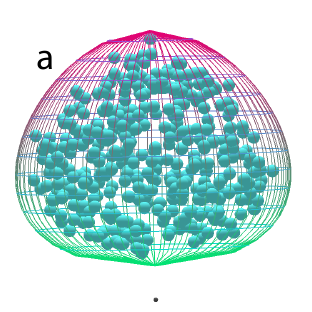
\includegraphics[scale=0.5]{img/colonization_1.png} 
\end{figure}
\begin{footnotesize}
\hfillŹródło: [1]
\end{footnotesize}
\end{frame}


\begin{frame}\frametitle{Algorytm kolonizacyjny}
\begin{itemize}
\item{Tworzenie węzłów drzewa do wszystkich atraktorów}
\end{itemize}
\begin{multicols}{2}
\begin{figure}
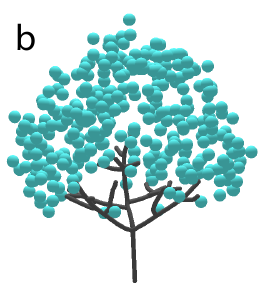
\includegraphics[scale=0.5]{img/colonization_2.png} 
\end{figure}
\begin{figure}
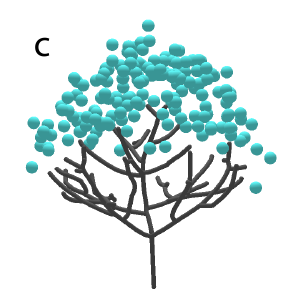
\includegraphics[scale=0.5]{img/colonization_3.png} 
\end{figure}
\end{multicols}
\begin{footnotesize}
\hfillŹródło: [1]
\end{footnotesize}
\end{frame}


\begin{frame}\frametitle{Algorytm kolonizacyjny}
\begin{itemize}
\item{Przetwarzanie (postprocessing) węzłów drzewa}
\end{itemize}\begin{multicols}{2}
\begin{figure}
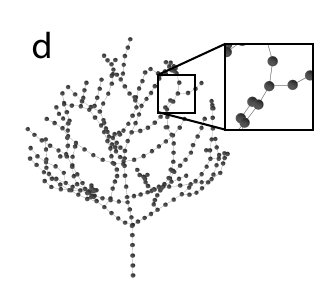
\includegraphics[scale=0.5]{img/colonization_4.png} 
\end{figure}
\begin{figure}
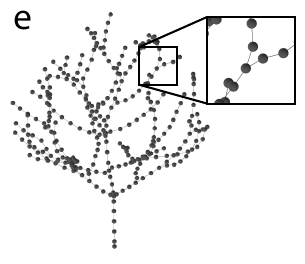
\includegraphics[scale=0.5]{img/colonization_5.png} 
\end{figure}
\end{multicols}
\begin{footnotesize}
\hfillŹródło: [1]
\end{footnotesize}
\end{frame}


\begin{frame}\frametitle{Algorytm kolonizacyjny}
\begin{itemize}
\item{Generowanie geometrii drzewa}
\item{Teksturowanie, dodanie liści}
\end{itemize}\begin{multicols}{3}
\begin{figure}
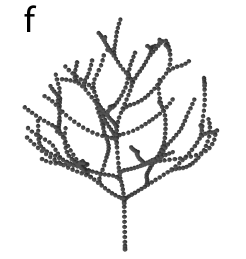
\includegraphics[scale=0.5]{img/colonization_6.png} 
\end{figure}
\begin{figure}
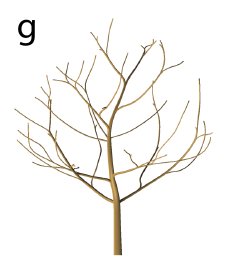
\includegraphics[scale=0.5]{img/colonization_7.png} 
\end{figure}
\begin{figure}
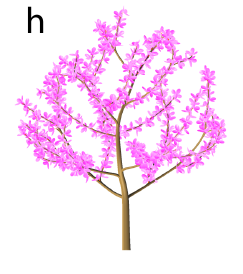
\includegraphics[scale=0.5]{img/colonization_8.png} 
\end{figure}
\end{multicols}
\begin{footnotesize}
\hfillŹródło: [1]
\end{footnotesize}
\end{frame}

\begin{frame}\frametitle{Algorytm kolonizacyjny}
\begin{itemize}
\item{Bardziej szczegółowo (przykład 2D)}
\end{itemize}
\begin{figure}
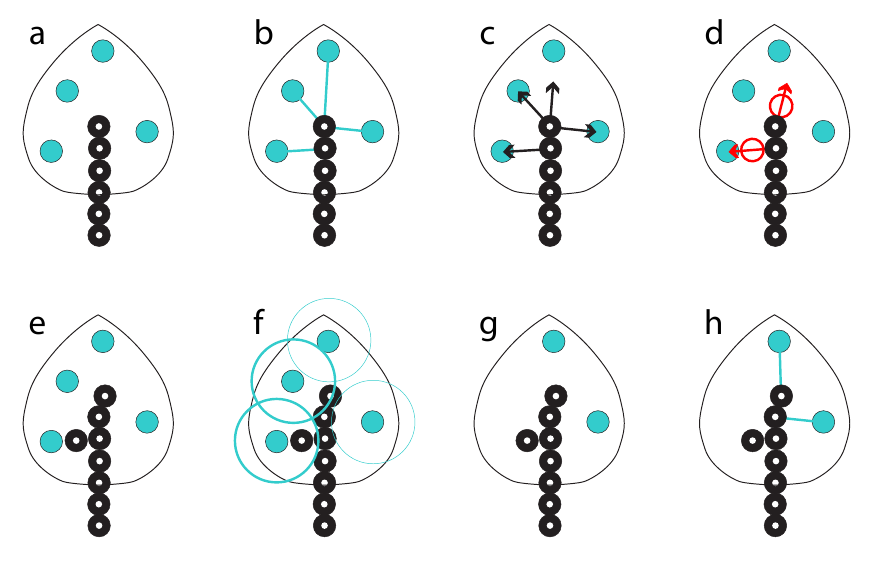
\includegraphics[scale=0.35]{img/colonization_9.png} 
\end{figure}
\begin{footnotesize}
\hfillŹródło: [1]
\end{footnotesize}
\end{frame}

\begin{frame}\frametitle{Źródła}
\begin{enumerate}
\item{Modeling Trees with a Space Colonization Algorithm}
\begin{itemize}
\item{Authors: A. Runions, B. Lane, P. Prusinkiewicz}
\end{itemize}
\end{enumerate}
\end{frame}

\end{document}